\section{Описание использованного алгоритма}

\subsection{Описание алгоритма подсчёта ряда по количеству членов}

\begin{figure}[H]
  \centering
  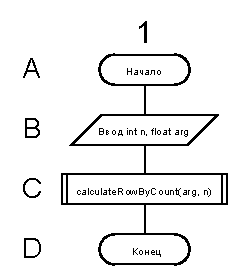
\includegraphics[width=0.25\textwidth]{fun_rows}
  \caption{Блок-схема алгоритма работы функции \texttt{main()} в библиотеке \texttt{rows}}
\end{figure}

\begin{figure}[H]
  \centering
  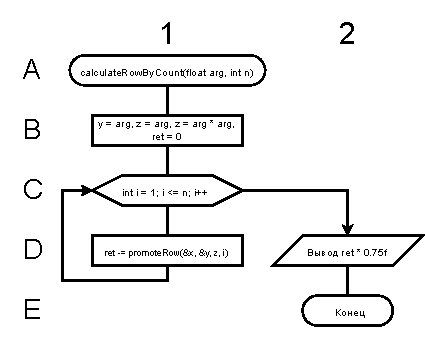
\includegraphics[width=0.45\textwidth]{fun_calculateRowByCount}
  \caption{Блок-схема алгоритма работы функции \texttt{calculateRowByCount()}}
\end{figure}

\subsection{Описание алгоритма подсчёта ряда по заданной точности}

\begin{figure}[H]
  \centering
  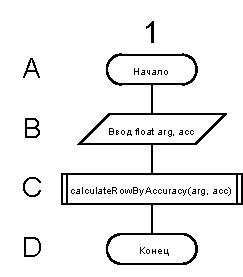
\includegraphics[width=0.25\textwidth]{fun_accuracy}
  \caption{Блок-схема алгоритма работы функции \texttt{main()} в библиотеке \texttt{accuracy}}
\end{figure}

\begin{figure}[H]
  \centering
  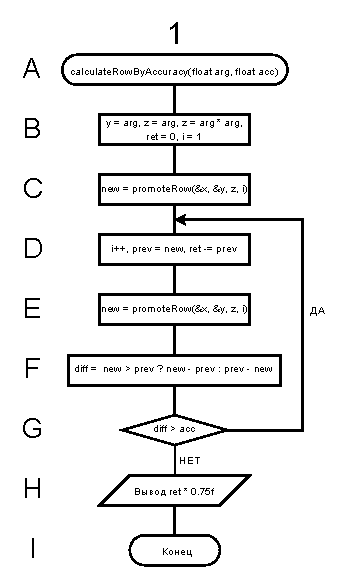
\includegraphics[width=0.45\textwidth]{fun_calculateRowByAccuracy}
  \caption{Блок-схема алгоритма работы функции \texttt{calculateRowByAccuracy()}}
\end{figure}

\subsection{Описание алгоритма общей части подсчёта ряда}

\begin{figure}[H]
  \centering
  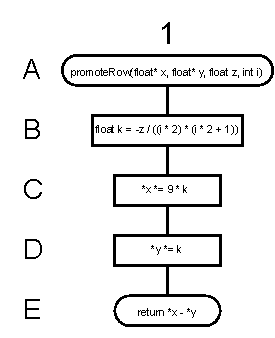
\includegraphics[width=0.35\textwidth]{fun_promoteRow}
  \caption{Блок-схема алгоритма работы функции \texttt{promoteRow()}}
\end{figure}
